% Figure from MATH 591 notes, section 12. Compile with the notes preamble.
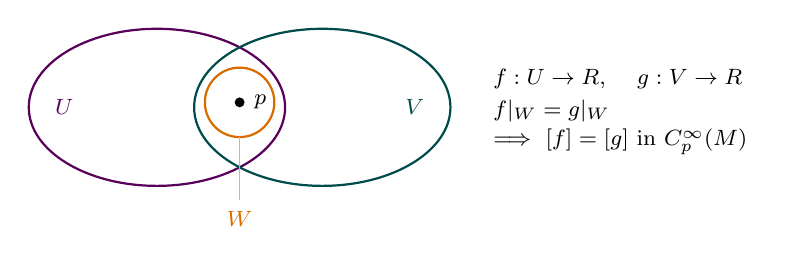
\begin{tikzpicture}[scale=1.05]
\draw[violet!70!black, thick] (0,0) ellipse (1.55 and 0.95);
\draw[teal!60!black, thick] (2.0,0) ellipse (1.55 and 0.95);
\node[violet!70!black,font=\footnotesize] at (-1.12,0) {$U$};
\node[teal!60!black,font=\footnotesize] at (3.12,0) {$V$};
\draw[orange!85!black, thick] (1.0,0.06) circle (0.42);
\draw[gray!55,thin] (1.0,-0.36) -- (1.0,-1.12);
\node[orange!85!black,font=\footnotesize,anchor=north] at (1.0,-1.14) {$W$};
\fill (1.0,0.06) circle (1.7pt);
\node[font=\footnotesize,anchor=west] at (1.06,0.06) {$p$};
\node[font=\footnotesize,anchor=west] at (3.95,0.34) {$f : U \to \mathbb{R}$, \quad $g : V \to \mathbb{R}$};
\node[font=\footnotesize,anchor=west] at (3.95,-0.04) {$f|_W = g|_W$};
\node[font=\footnotesize,anchor=west] at (3.95,-0.42) {$\Longrightarrow\ [f] = [g]$ in $C_p^\infty(M)$};
\end{tikzpicture}
